\chapter{Information-Driven Subword Tokenisation}\label{chapter:infotokenisation}

Modern LM architectures use a subword-based input representation --- orthographic split into subword tokens using subword tokenisation, as introduced in \cref{sec:12-subword}. Subword tokenisation purportedly offers a balance between processing raw bytes and processing full words by being computationally efficient, gracefully handling OOV issues and maintaining a reasonable vocabulary size. Despite these advantages, there have been many criticisms of popular subword tokenisation algorithms like \bpe and WordPiece, as described in \cref{sec:12-subwordlimitations}. In particular, since these methods are fully data-driven and based on compression, they do not tend to group characters or bytes into sequences that align with linguistic units like morphemes --- a limitation which has been theorised to lead to worse performance particularly for multilingual language modelling. Another limitation is reliance on a fixed vocabulary size --- in order to address this limitation, recent work on tokenisation has proposed operating directly on bytes and using \textbf{patching} to dynamically group byte sequences during training.

This chapter explores a connection between patching and the unsupervised word segmentation methods presented in \cref{chapter:phonology}. This connection, described below in \cref{sec:16-motivation}, is used to inspire a novel subword tokenisation method, \bytespan, as introduced in \cref{sec:16-bytespan}.  Experiments compare \bytespan to \bpe for English and in a multilingual setting; the experimental setup is described in \cref{sec:16-setup} and results are presented in \cref{sec:16-results}. Driven by grouping predictable sequences of bytes, rather than compression, the vocabulary learned by \bytespan contains subwords that more closely align with morphemes, without sacrificing compression. Finally, a broader discussion of these results is provided in \cref{sec:16-discussion}.

% Intrinsic results show that our method yields higher morphological alignment scores and higher \renyi efficiency scores for most vocabulary sizes, without compromising compression. Our multilingual experiments show similar \renyi efficiency and fertility to \bpe across 25 languages and we propose methods for balancing a vocabulary to efficiently tokenise rare orthographies. 

% Recent dynamic tokenisation methods operate directly on bytes and pool their latent representations into \textit{patches}. This bears similarities to computational models of word segmentation that determine lexical boundaries using spikes in an autoregressive model's prediction error. Inspired by this connection, we explore whether grouping predictable bytes---rather than pooling their representations---can yield a useful fixed subword vocabulary. We propose a new information-driven subword tokeniser, \bytespan, that uses an external byte-level LM during training to identify contiguous predictable byte sequences and group them into subwords. Experiments show that \bytespan yields efficient vocabularies with higher morphological alignment scores than \bpe for English. Multilingual experiments show similar compression and \renyi efficiency for \integer{25} languages. 

\section{Motivation}\label{sec:16-motivation}

To remove the LMs' dependence on tokenisers while preserving computational efficiency, recent work on tokenisation proposes to operate directly on bytes and pool their representations into \textit{patches}. These patches are created either by pooling fixed-length spans (\citealp{dai-etal-2020-funnel, nawrot-etal-2022-hierarchical, yu2023megabyte}, \textit{inter alia}) or by dynamically pooling predictable byte sequences within a context window \citep{nawrot-etal-2023-efficient, pagnoni2024byte}, as introduced introduced in \cref{sec:12-alternative}.

The subword tokenisation method proposed in this chapter relates to the work of \citet{pagnoni2024byte}, who group bytes into dynamic `patches' according to their entropies, as given by a byte-level LM. They experiment with two methods to identify patch boundaries; their \textbf{global constraint} identifies bytes whose entropies exceed a fixed threshold and their \textbf{monotonic constraint} identifies bytes whose entropies decrease monotonically. A \textbf{patching function} then segments a stream of bytes into patches that are fed through a latent transformer, with predicted patches decoded by the smaller byte-level LM. Conceptually, this smaller LM can make the relatively `easy' next-byte predictions given the low entropy of each byte within the patch.

The global constraint closely resembles the \emph{threshold strategy} for unsupervised word segmentation introduced in \cref{sec:15-wordsegunsupervised} --- grouping tokens that fall under a threshold is equivalent to placing boundaries where tokens exceed a threshold. Additionally, \citet{pagnoni2024byte} use per-token \emph{entropy} to determine how bytes are grouped, one of the four signals explored for unsupervised word segmentation in \cref{sec:15-wordsegunsupervised}. More generally there are clear parallels between dynamic patching, subword tokenisation and unsupervised word segmentation --- all seek to group consecutive tokens, whether it be characters within a word to create subwords, bytes within a span to create patches, or phonemes within an utterance to identify words. Where standard subword algorithms like \bpe differ from dynamic patching and unsupervised word segmentation is that the former is data-driven, using only frequency to group items, whereas the later use predictability measures derived from a language model. Just as many unsupervised word segmentation algorithms are based on the simple principle that predictability within lexical units is high, and predictability between lexical units is low \citep{harris1955} --- using this principle to try to identify words --- dynamic patching uses the same principle, but to group bytes in a manner that can then be easily re-constructed to reduce error when language modelling. 

There are clear parallels between dynamic patching and the unsupervised word segmentation methods introduced in \cref{sec:15-wordsegunsupervised}. In particular, the \emph{threshold strategy} closely resembles the global constraint of \citet{pagnoni2024byte} --- grouping tokens that fall under a threshold is equivalent to placing boundaries where tokens exceed a threshold. In both cases, per-token \emph{entropy} is used to create a signal over tokens.

Dynamic patching relies on trainable model components, a practice that unwittingly mirrors computational models of word segmentation. In both fields, methods draw on the simple principle that predictability within lexical units is high, and predictability between lexical units is low \citep{harris1955}. For word segmentation, this is used to inspire methods for how children may learn to segment speech, as introduced in \cref{sec:12-wordseg} and in \cref{chapter:phonology}, where new unsupervised methods were implemented using the predictions from phoneme LMs. In dynamic patching, the principle is used to group predictable bytes into, again using the predictions of a byte-level LM. 

Inspired by this connection, this chapter explores whether grouping predictable bytes using methods inspired by word segmentation can yield a useful fixed subword vocabulary. A new information-driven tokeniser is introduced, \bytespan, which uses an external byte-level LM to identify predictable contiguous byte sequences, using entropy or surprisal as measures of information. Byte spans are identified using a global threshold constraint, a monotonic constraint, or a combination of the two, and several methods are used for creating a subword vocabulary from identified byte spans. These methods are used to train English and multilingual tokenisers which are compared to \bpe across vocabulary sizes. 


% \zeb{I'm not sure this paragraph fits here, maybe we move this to the discussion?} Our proposed approach is also related to work on \textbf{dynamic tokenisation} (e.g., \citet{feher2024retrofitting}) that adaptively adjusts token boundaries using an update function \(\mathcal{U}\) to update an initial tokeniser \(<\mathcal{V}_{\text{init}}, \mathcal{T}_{\text{init}}>\): 
% \[ \mathcal{T}_{\text{new}} (\mathcal{D}) =  \mathcal{U} (\mathcal{T}_{\text{new}} (\mathcal{D})  )\]


Where these methods differ is in the input representation. Whereas the word segmentation methods operate over unsegmented phonemes, patching typically operates over orthographic text split into bytes (including word boundaries). Additionally, \citet{pagnoni2024byte} only use entropy as a cue, whereas \cref{sec:15-wordsegunsupervised} also explored the use of loss, rank and utterance boundary probability.

Although \citet{pagnoni2024byte} found that dynamic patching improved computational efficiency for LLMs, it does require a more sophisticated architecture where a byte-level LM must be utilised during training and inference. It is of interest to establish whether this idea of grouping predictable bytes could be applied to a static tokeniser, where creating a fixed vocabulary is a pre-processing step that occurs before model training. Given that related unsupervised word segmentation methods successfully identified word-like units in child-directed speech across 31 languages, this chapter explores whether the same principle can be successfully applied to learn a subword vocabulary in a standard language modelling setup. 

% We draw parallels between these patching constraints and computational models of word segmentation. These models are designed to demonstrate how distributional information could be leveraged by language-learning infants to bootstrap a vocabulary, following the influential statistical learning experiments of \citet{Saffran1996learning} who observed this ability in young infants. In the typical framework, these models use unsupervised algorithms to group unsegmented sequences of phonemes from transcriptions of child-directed speech into word-like units. One approach involves maximising the likelihood of word-level \ngram models(e.g., \citealp{Brent1999, Venkataraman2001}), a method that closely resembles the UnigramLM tokenisation algorithm \citep{kudo-2018-unigram}. Another approach is to extract measures of uncertainty using phoneme-level \ngram models and posit boundaries where these measures spike or surpass a threshold (e.g., \citealp{ccoltekin2014explicit, goriely2023word}). Neural language models have also been used, for instance by using the prediction of an utterance boundary (which is included in the phoneme sequence) to posit a word boundary \citep{christiansen1998learning}. In a formative analysis of character-level RNNs, \citet{elman1990finding} noted that the prediction error from a neural language model could serve as a cue for lexical boundaries more broadly; boundaries around words, morphemes, but also frequent multi-word sequences, which children often treat as fixed lexical items \citep{macwhinney1978}. Based on this observation, \addcites trained phoneme-level GPT-2 LMs across 31 languages and demonstrated a method for extracting word boundaries from the trained models; computing model uncertainty using entropy, rank and surprisal from the predictions at each point and segmenting at points of high uncertainty. These information-based approaches to word segmentation, and the later study in particular, closely resemble the patching constraints of \citet{pagnoni2024byte}.

% We hypothesise that a modular tokenisation pipeline using constraints based on byte-level information might retain the conceptual advantages of patch-based approaches while retaining the benefits of creating a fixed vocabulary as a pre-processing step before training. By drawing parallels with computational models of word segmentation, we hypothesise that the resulting subword tokens align better with morphological segmentations of natural language than compression-based methods such as \bpe.


\section{ByteSpan subword tokenisation}\label{sec:16-bytespan}

\bytespan uses an external byte-level LM during training to identify predictable byte sequences and group them into subwords. During inference, the resulting vocabulary can be paired with any standard tokenisation function (e.g., longest-prefix match) and used with any modern LM architecture. % (e.g., \citealp{touvron-2023-llama}) without modifications. 

\begin{figure}[!t]
    \centering
    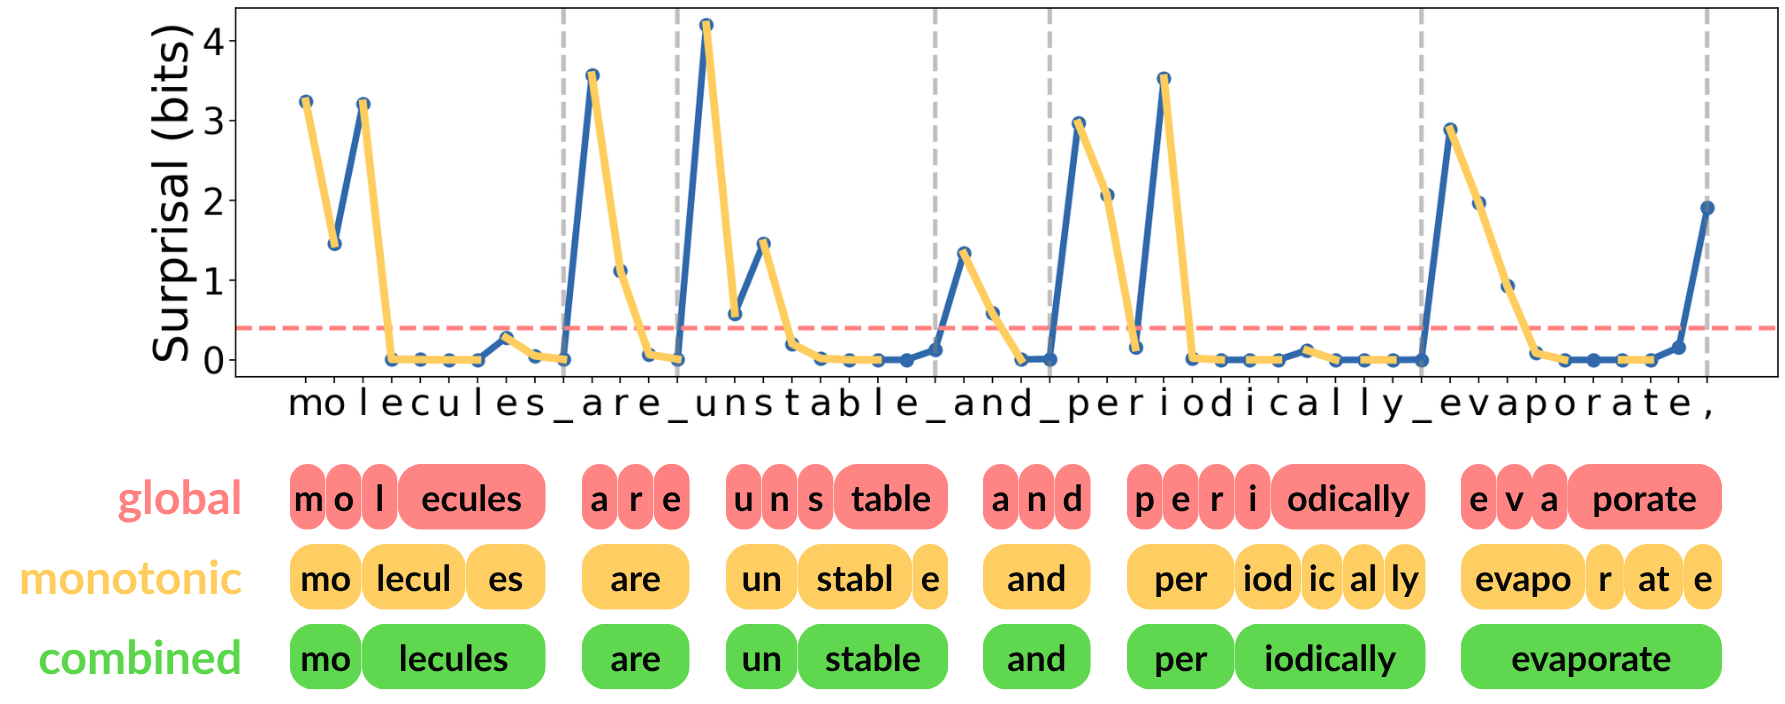
\includegraphics[width=0.8\linewidth]{16InfoTok/example.png}
    \caption{\textbf{Information-Driven Subword Creation.}
    Per-byte \textbf{surprisal} of \textit{\enquote{molecules are unstable and periodically evaporate}} from a byte-level LM. \bytespan groups contiguous bytes using one of three constraints; the \red{global constraint} uses a fixed threshold, the monotonic constraint groups bytes with decreasing information and the combined constraint groups bytes that meet either constraint. Grey vertical lines indicate pre-tokenisation boundaries.
    }
    \label{fig:16-example}
\end{figure}

\bytespan works by first collecting predictions from a byte-level LM over a corpus, from which key statistics are calculated. The algorithm then groups contiguous sequences of bytes using a constraint based on these statistics.

\paragraph{Statistics and constraints.} Following \citet{pagnoni2024byte}, per-byte \textbf{entropy} \(H(\ch_i)\) Two constraints are considered, per-byte \textbf{entropy} \(H(\ch_i)\) and per-byte \textbf{surprisal} \(s(\ch_i)\).\footnote{Surprisal is equivalent to the `loss' measure used in the previous chapter} Based on the constraints used by \citet{pagnoni2024byte}, two constraints are implemented. For example, using entropy, these are:


Following \citet{pagnoni2024byte}, per-byte \textbf{entropy}\footnote{Note that \citet{pagnoni2024byte} actually use \emph{next-byte} entropy, which would shift byte spans by one unit.} \(H(\ch_i)\) is used as a key statistics, with which two constraints are used to identify byte spans: 
\begin{align}
    \mathrm{\defn{Global~Constraint}} &~~ H(\ch_t) < \thres_g \\
    \mathrm{\defn{Monotonic~Constraint}} &~~ H(\ch_t) - H(\ch_{t-1}) < 0 
\end{align}

The first constraint groups bytes that fall under a fixed global threshold and the second constraint groups byte with monotonically decreasing information. These are visualised in \cref{fig:16-example}, where for instance the global constraint segments the word \ex{unstable} as $\{\ex{u}, \ex{n}, \ex{s}, \ex{table} \}$ whereas the monotonic constraint produces $\{\ex{un}, \ex{stabl}, \ex{e}\}$. The algorithm for segmenting a sequence using the monotonic constraint is provided in \emph{Algorithm} \ref{alg:1}. Each byte is processed once in a single pass through the sequence, so the complexity is \(O(n)\). 

In addition to entropy, \textbf{surprisal} is also considered as an information signal, noting that \bytespan is compatible with any function mapping from the LM's logits to a scalar. A third constraint is also considered, one that that combines the global constraint with the monotonic constraint, grouping contiguous bytes that meet either. This follows from the observation that the monotonic constraint can become unstable when the entropy or surprisal of a byte is close to zero. This can be seen from the small increase in surprisal from \ex{l} to \ex{e} causing \ex{stable} to be split into two units in the example given in \cref{fig:16-example}. In such cases, the \defn{combined constraint} joins segments below a low threshold \(\thres_g \) with monotonically decreasing segments, potentially preventing these unwanted segmentations.

% \zeb{improve this}
% Conceptually, the global constraint should capture highly predictable sequences, whereas we anticipate that the monotonic constraint will capture morphological or lexical units, following \citet{elman1990finding}'s observations that model uncertainty spikes at such boundaries, later utilised by as a strategy by word segmentation models.

The global constraint aims to capture highly predictable sequences. However, it often results in splitting words into single byte tokens followed by the remainder of the word, whereas the monotonic constraint is superior at recovering morphological and lexical units. This follows \citet{elman-1990-finding}'s observations that model uncertainty typically spike at such boundaries.

\begin{algorithm}[t]
\caption{\textbf{ByteSpan Tokenisation}}
\begin{algorithmic}[1]
\STATE \textbf{Input:} Byte sequence $X = \ch_1, \ch_2, \dots, \ch_n$, Byte-level entropy values $H(\ch_i)$
\STATE \textbf{Output:} Tokenised sequence $T$
\STATE Initialise $i \gets 2$ \COMMENT{Start of the byte sequence}
\STATE Initialise $T \gets []$ \COMMENT{Empty tokenised sequence}

\WHILE{$i \leq n$}
    \STATE $j \gets i$
    \WHILE{$j \leq n$ \textbf{and} $H(\ch_j) - H(\ch_{j-1}) < 0$}
        \STATE $j \gets j + 1$
    \ENDWHILE
    \STATE Extract segment $\ch_i, \ch_{i+1}, \dots, \ch_{j}$
    \STATE Append the segment to $T$
    \STATE $i \gets j$
\ENDWHILE

\STATE \textbf{Return:} $T$
\end{algorithmic}
\label{alg:1}
\end{algorithm}

\paragraph{Learning a vocabulary.} Three methods are proposed for using these constraints to learn a fixed-size vocabulary \(V\) from a training corpus $\dataset = \{\chvec_n\}_{n=1}^N$:
\begin{enumerate}
    \item \textbf{Frequency:} Using any of the three constraints, identify all unique subwords in the training corpus. Sort the subwords by frequency and use the top \(|V|\) as the tokeniser's vocabulary.
    \item \textbf{Incremental:} Using the global constraint, gradually increase $\thres_g$ until the desired vocabulary size is reached. To prevent rare subwords from being added to the vocabulary, a minimum frequency threshold $\thres_f$ can also be applied.
    \item \textbf{Seeding \bpe:} Using any of the three constraints, apply the \textbf{frequency cut-off} method to learn a portion $p\%$ of the final vocabulary, then apply \bpe to learn the rest of the vocabulary. 
\end{enumerate}

The frequency method is the most efficient, requiring only a single pass of the training dataset. However, for the global constraint, it requires pre-determining the global threshold $\thres_g$. The incremental method gets around this limitation by gradually increasing the threshold until the desired vocabulary size is reached. Unlike the other methods, this means that vocabularies with a larger \(|V|\) will not necessarily contain the vocabularies of tokenisers trained with a small \(|V|\). This is because higher thresholds lead to the \textbf{absorption} (or subsumption) of constituent subsequences. For instance, increasing the threshold in \cref{fig:16-example} would lead to $\ex{nstable}$ replacing $\ex{table}$ in the vocabulary.

In theory, the incremental method is also compatible with the combined constraint, but in practice, the number of subwords identified by the monotonic constraint exceeds most desired vocabulary sizes at the first pass, causing the algorithm to terminate immediately without the global constraint applying.

Finally, the seeding method could provide a trade-off between \bytespan and \bpe by first identifying predictable multi-byte units and then using \bpe to efficiently compress frequently co-occurring units. Note that setting $p=100\%$ is equivalent to the frequency method and that setting  $p=0\%$ is equivalent to just using \bpe to learn the vocabulary.

\paragraph{ByteSpan vs BPE.}

Unlike \bpe, which merges tokens incrementally based on frequency, \bytespan finds contiguous low-information segments. The vocabulary-learning methods are flexible, achieving a target vocabulary size by either incrementally increasing the information threshold to include longer and less predictable sequences, or by trimming down a large set of discovered units according to frequency.

By only including the longest subsequences determined by the constraints used, intermediate merges are avoided, unlike \bpe. Since a sequence cannot be decomposed using a recursive \bpe-style inference procedure, \textbf{longest-prefix matching} is used as the the inference procedure, as used by WordPiece (\wordpiece, \citealp{schuster-nakajima-2012-voice}). Notably, \bytespan can also group beyond word boundaries and create \defn{superwords} (e.g., if the threshold were raised in \cref{fig:16-example}, \ex{nstable and} could be added as a single token). The implementation ensures that learned subwords align with \bpe pre-tokenisation constraints by preventing subwords from crossing pre-tokenisation boundaries (the vertical lines in \cref{fig:16-example}).

\paragraph{ByteSpan vs Patching.}
% \zeb{this paragraph needs work}
\bytespan retains the information-driven approach of patching while preserving the computational benefits of keeping tokenisation separate from language modelling. In particular, it eliminates the additional complexity of batching in patch-based methods (e.g., where patch boundaries do not align across sequences). The method only requires computing the entropy (or surprisal) of bytes once in order to learn a fixed \(\mathcal{V}\) before training, which can then be used by standard LMs with any corpus, whereas the patching method of \citet{pagnoni2024byte} requires a byte-level LM to compute the entropy of every byte seen during training. Unlike \bytespan, patching does not create a fixed size vocabulary, as patches are dynamically created during training.

\section{Experimental setup}\label{sec:16-setup}

The information-driven tokenisation approach is explored in both English and multilingual settings. Below, the experimental setup is described.

\paragraph{Data.} 
English tokenisers are trained on a sample of the \fineweb dataset\footnote{\href{https://huggingface.co/datasets/HuggingFaceFW/fineweb-edu}{\myemph{huggingface.co/datasets/HuggingFaceFW/fineweb-edu}}.} \citep{penedo2024finewebdatasetsdecantingweb}.
For the multilingual tokenisers, a balanced \integer{25}-language sample from the \commoncorpus \footnote{\href{https://huggingface.co/datasets/PleIAs/common_corpus}{\myemph{huggingface.co/datasets/PleIAs/common_corpus}}.} \citep{common_corpus} is used, with languages selected for morphological diversity. Each corpus is converted into bytes using the Huggingface \texttt{ByteLevel} pre-tokeniser and split each corpus into three equal subsets: one to train the byte-level model, one to train the tokenisers, and one for evaluation. The \fineweb subsets contain approximately \q{500}{\million} bytes and the \commoncorpus subsets contain approximately \q{250}{\million} bytes (\q{10}{\million} per language).

\paragraph{Byte-level Model.} 

\begin{table}[t]
    \centering
    \small
    \begin{tabular}{lr}
        \toprule
        Parameter & Value \\
        \midrule
        Architecture & \llama-2 \\
        Layers & 6 \\
        Attention Heads & 24 \\
        Embedding Size & 768 \\
        Inner Size & 3072 \\
        \midrule
        Max Example Length & 2048 \\
        Learning Rate & 0.0006 \\
        Optimiser & AdamW \\
        Scheduler Type & Warm-up stable decay \\
        Max Steps & 50k \\
        Warm-up Steps & 2k \\
        Batch Size & 128 \\
        \bottomrule
    \end{tabular}
    \caption{Hyperparameter settings for training the \llama byte-level model. Where values are not reported, they may be assumed to be default values.}
    \label{tab:16-trainingparams}
\end{table}

% The byte-level LM is based on the \llama-2 architecture \citep{touvron-2023-llama} and is used to collect the contextual surprisal and entropy for each byte in the corpora. The byte-level statistics only need to be collected once and can be reused for each tokeniser setup.

A small byte-level LM is trained on the subsets of the \fineweb and \commoncorpus datasets. The model and training parameters are provided in \cref{tab:16-trainingparams} --- these follow the parameters used by \citet{lesci2025causal}, who explore the causal effect of tokenisation on how LMs assign probability to token sequences. The \llama architecture is used instead of \gpt since it is more representative of modern LM training, whereas \gpt is appropriate for architectural and phonological experimentation.

% The \llama-2 architecture is used with \integer{24} attention heads, \integer{6} layers, hidden size of \integer{768}, and tied input--output embeddings, totalling \q{57}{\million} parameters.
% The optimiser used is AdamW \citep{adam,loshchilov2018decoupled}, with learning rate \snum{6e-4}, parameters $\beta_1\mathop{=}0.9$, $\beta_2\mathop{=}0.95$, $\epsilon\mathop{=}\snum{1e-8}$, and weight decay set to \float{0.1}.
% The warm-up-stable-decay schedule is used \citep{zhai2022scaling}, where after warm-up, the learning rate stays constant for most training and decreases briefly during the cool-down. Unlike the cosine schedule, this approach does not need a pre-specified compute budget, facilitating continued training and enhancing our artifact's value for the community. It is also more effective for small language models \citep{hu2024minicpm, wen2024understanding}.
% During training, the context size is set to \integer{2048} tokens and the batch size is set to \integer{128}, clip the norm of the gradients to \float{1}, and train for \q{50}{\thousand} steps, saving checkpoints every \q{2}{\thousand} steps.
% Each model is trained with the same seed so that data order and parameter initialisation is consistent across experiments.

The English and multilingual byte-level models are then used to extract per-byte entropy and surprisal. This is done on separate subsets of \fineweb and \commoncorpus to prevent over-fitting. Using a context size of \integer{2048}, the data is shifted along by strides of \integer{512}. This ensures that all byte-level predictions have at least \integer{1536} tokens of context. The logits at each byte are then used to calculate surprisal and entropy. These predictions are stored as a Huggingface dataset to facilitate training tokenisers using \bytespan.

\paragraph{Tokeniser Setup.} 
For the English tokenisers, a suite of tokenisers is trained across three vocabulary sizes; \q{16}{\thousand}, \q{32}{\thousand} and \q{64}{\thousand}. For the multilingual setting, a vocabulary size of \q{128}{\thousand} is used. For each vocabulary size, tokenisers are trained using the three constraints and two measures (entropy and surprisal). For the global constraint, the incremental method is used to learn a vocabulary with a minimum frequency threshold $\thres_f = 20$. For the monotonic constraint, the frequency method and the seeding method are used, setting $p=50\%$. The same methods are used for the combined constraint, with the global threshold $\thres_g$ set to be the 30th-percentile entropy (or surprisal) in the data.

As baselines, \bpe tokenisers are trained for each vocabulary size and corpus. Additionally, \bpe tokenisers that use WP-style inference are trained to match the inference procedure of the \bytespan tokenisers, since inference can have a significant impact on intrinsic tokeniser evaluation, as shown in \cref{sec:12-subwordmethods}. There are labelled \bpewp.\footnote{The WordPiece tokeniser trainers on Huggingface actually use \bpe, not the WordPiece objective, to learn their vocabularies.}

The \bytespan tokenisers (and \bpewp) are initialised with three copies of every byte in their vocabularies. In addition to each byte, these are the byte with the WordPiece \textbf{continuation prefix} \texttt{\#\#} (used by the inference method to distinguish pre-token-internal tokens from pre-word-initial tokens) and the byte with the start-of-word prefix (used by the \texttt{ByteLevel} pre-tokeniser to indicate whitespace). This slightly wastes vocabulary space compared to \bpe, as 768 base tokens are required instead of 512, but is a consequence of the complexities of combining tokeniser modules.

\paragraph{Intrinsic Evaluation.} 

The intrinsic evaluation benchmark of \citet{uzan-etal-2024-greed} is used for evaluating the tokenisers. It consists of four information measures: Morphological Alignment, Cognitive Plausibility, \renyi Efficiency, and Fertility:

\begin{itemize}[leftmargin=*]
    \item \textbf{Morphological alignment} The alignment of tokenisers with gold-standard morphological segmentations of words. The benchmark compares tokeniser alignment to morphological annotations from seven resources and returns a macro-averaged $F_1$ score. The morphological data comes from LADEC \citep{gagne2019ladec}, MorphoLex \citep{sanchez2018morpholex}, MorphyNet \citep{batsuren-etal-2021-morphynet}, and DagoBert \citep{hofmann-etal-2020-dagobert}. \citet{uzan-etal-2024-greed} further augment these datasets with morpheme segmentation data \citep{batsuren-etal-2022-unimorph}, novel blend structure detection data \citep{pinter-etal-2021-will}, and compound separation data \citep{minixhofer-etal-2023-compoundpiece}.
    \item \textbf{Cognitive plausibility} A benchmark from \citet{beinborn-pinter-2023-analyzing} who found that human reaction time and accuracy from a lexical decision task correlated negatively with the number of tokens produced by a tokeniser for words, and correlated positively for non-words. The score consists of an average from correlation scores across the four conditions (words/non-words, accuracy/reaction time) with a higher score indicating increased `cognitive plausibility'.
    \item \textbf{\renyi efficiency} A measure that penalises vocabularies consisting of many low-frequency or high-frequency tokens. It captures efficient channel usage and was found to correlate highly with \myemph{Bleu} scores \citep{zouhar-etal-2023-tokenization}.
    \item \textbf{Fertility} The average number of subwords produced per tokenised word, used by \citet{acs2019exploring} to compare compression efficiency across languages for a multilingual tokeniser. A score of \integer{1} indicates perfect compression; every word in the evaluation set exists in the tokeniser's vocabulary.
\end{itemize}

This setup allows tokenisers to be evaluated without the time- and resource-intensive process of training and evaluating LMs on downstream tasks. In their study, \citet{uzan-etal-2024-greed} use \minipile \citep{kaddour2023minipile} to compute \renyi efficiency and fertility --- matching the dataset used to train their tokenisers. To match the training data used here, these measures are computed using the third subsets of the prepared corpora (\fineweb for English, \commoncorpus for the multilingual tokenisers). For the multilingual tokenisers, only \renyi efficiency and fertility using \commoncorpus are reported, as the intrinsic evaluation benchmark for the other metrics only support English.

\paragraph{Extrinsic Evaluation.} 

Whereas intrinsic evaluation of tokenisers involves using metrics computed from their vocabularies or tokenised corpora, extrinsic evaluation explores the effect that tokenisers have on language modelling tasks. In order to evaluate the capabilities of language models trained with \bytespan, \llama models are trained on the largest English tokenisers (those with a vocabulary size of \q{64}{\thousand}). For the \bytespan tokenisers, surprisal is used as the information signal. The same training configuration is used as the byte-level models, as described in \cref{tab:16-trainingparams}\footnote{The only difference in implementation is that models are trained using 4GPUs, each with a batch size of \integer{32} --- but the effective batch size is still \integer{128}.}, and the models are trained on the entirety of \fineweb (training ends before any data is repeated).

The resulting models are then evaluated using \blimp, first introduced in \cref{sec:12-blimp}. Additionally, the model loss on a held-out validation set is used to compute \textbf{bits per byte} (BPB). Formally, BPB is computed as follows:

\begin{align}
    \mathrm{BPB} &= \frac{|\mathrm{tokens}|}{|\mathrm{bytes}|} \times \frac{\ln(\mathrm{PPL})}{\ln{2}},
\end{align}

where PPL is perplexity, computed by averaging the negative log likelihoods (NLL) given by the language model at each position $n$ in the validation data:

\begin{align}
    \mathrm{PPL} &= \exp{\left(\frac{1}{N} \sum_{n=1}^{N}{\mathrm{NLL}_n} \right)}.
\end{align}

BPB provides a means of comparing the perplexities assigned by models that use different tokenisers  \citep{choe2019bridging}. This is because PPL provides the average perplexity for each token in the sequence, but the total information in a sequence should be independent of segmentation. Hence, BPP normalises perplexity by the average number of tokens per byte, making it a tokeniser-independent measure of language modelling performance. During the calculation of PPL, each validation instance is truncated to \integer{2048} bytes, since this provides an upper bound for the number of tokens, ensuring that each example fits into the context window of any model.

% Whereas intrinsic evaluation of tokenisers involves using metrics computed from their vocabularies or tokenised corpora, extrinsic evaluation explores the effect that tokenisers have on language modelling tasks. As an initial experiment, we train three models using \bpe and three models using \bytespan-S at vocabulary size \q{32}{\thousand}. The model parameters and training procedure are the similar to the byte-level models, as described in \cref{app:implementation_details}. The only differences are that we use 4 GPUs (the effective batch size is kept the same) and we train on all of \fineweb (no data is repeated during training).

\section{Results}\label{sec:16-results}


\setlength{\tabcolsep}{5pt}
\begin{table}[t]
    \centering
    \footnotesize
    \begin{tabular}{cccccccc}
        \toprule
        Vocab Size & Tokeniser & Constraint & \makecell{Learning \\ Method} & \makecell{Morph. \\ Alignment} & \makecell{Cognitive \\ Plausibility} & Fertility & \makecell{Renyi \\ Efficiency} \\
        \midrule
        % \multirow{6}{*}{\integer{8064}} & BPE & - & - & .726 & \textbf{.262} & 1.34 & .516 \\
        %  & BPE-WP      &     -         & - & .841 & .256 & \textbf{1.32} & .526 \\
        %  & ByteSpan  & \red{Global} & Increment  & .883 & .137 & 2.22 & .469 \\
        %  & ByteSpan  & \yellow{Monotonic} & Seeding & .884 & .242 & 1.35 & \textbf{.530} \\
        %  & ByteSpan  & \green{Combined} & Seeding & .867 & .244 & 1.34 & .528 \\
        %  & ByteSpan  & \yellow{Monotonic} & Frequency & .878 & .220 & 1.50 & \textbf{.530} \\
        %  & ByteSpan  & \green{Combined} & Frequency & \textbf{.895} & .237 & 1.42 & .524 \\
        % \midrule
        \multirow{12}{*}{\q{16}{\thousand}} & BPE  & - & - & .694 & \textbf{.302} & 1.21 & .468 \\ 
        & BPE-WP & - & - & .834 & .297 & \textbf{1.19} & .472 \\ 
        & ByteSpan-S & \red{Global} & Increment & \textbf{.899} & .146 & 1.90 & .470 \\ 
        & ByteSpan-E & \red{Global} & Increment & \textbf{.899} & .146 & 1.90 & .470 \\ 
        & ByteSpan-S  & \yellow{Monotonic} & Frequency & .885 & .254 & 1.39 & \textbf{ .483} \\ 
        & ByteSpan-E & \yellow{Monotonic} & Frequency & .882 & .271 & 1.38 &  .482 \\ 
        & ByteSpan-S & \yellow{Monotonic} & Seeding & .862 & .272 & 1.22 & .476 \\
        & ByteSpan-E  & \yellow{Monotonic} & Seeding & .857 & .273 & 1.22 & .476 \\
        & ByteSpan-S  & \green{Combined} & Frequency & .890 & .268 & 1.29 & .477 \\ 
        & ByteSpan-E & \green{Combined} & Frequency & .889 & .286 & 1.27 & .476 \\ 
        & ByteSpan-S  & \green{Combined} & Seeding & .867 & .279 & 1.21 & .474 \\
        & ByteSpan-E & \green{Combined} & Seeding & .866 & .281 & 1.21 & .474 \\
        \midrule
        \multirow{12}{*}{\q{32}{\thousand}} & BPE & - & - & .648 & \textbf{.344} & 1.13 & .427 \\
        & BPE-WP  & - & - & .821 & .337 & \textbf{ 1.11} & .431 \\
        & ByteSpan-S & \red{Global} & Increment      & \textbf{.890} & .192 & 1.46 & .466 \\
        & ByteSpan-E & \red{Global} & Increment      & \textbf{.890} & .193 & 1.48 & \textbf{.467} \\
        & ByteSpan-S  & \yellow{Monotonic} & Frequency   & .843 & .277 & 1.31 & .446 \\
        & ByteSpan-E & \yellow{Monotonic} & Frequency   & .837 & .291 & 1.30 & .445 \\
        & ByteSpan-S & \yellow{Monotonic} & Seeding & .862 & .314 & 1.13 & .433 \\
        & ByteSpan-E  & \yellow{Monotonic} & Seeding & .859 & .315 & 1.13 & .433 \\
        & ByteSpan-S & \green{Combined} & Frequency    & .865 & .295 & 1.20 & .438 \\
        & ByteSpan-E  & \green{Combined} & Frequency    & .854 & .308 & 1.19 & .438 \\
        & ByteSpan-S & \green{Combined} & Seeding  & .860 & .318 & 1.12 & .432 \\
        & ByteSpan-E  & \green{Combined} & Seeding  & .858 & .322 & 1.12 & .432 \\
        \midrule
        \multirow{12}{*}{\q{64}{\thousand}} & BPE & - & - & .609 & \textbf{.362} & 1.09 & .395 \\ 
        & BPE-WP & - & - & .773 & .358 & \textbf{1.06} & .399 \\ 
        & ByteSpan-S  & \red{Global} & Increment & \textbf{.865} & .258 & 1.18 & .421 \\ 
        & ByteSpan-E  & \red{Global} & Increment & \textbf{.865} & .271 & 1.20 & \textbf{.424} \\ 
        & ByteSpan-S & \yellow{Monotonic} & Frequency & .816 & .285 & 1.25 & .416 \\ 
        & ByteSpan-E  & \yellow{Monotonic} & Frequency & .806 & .293 & 1.24 & .416 \\ 
        & ByteSpan-S  & \yellow{Monotonic} & Seeding & .809 & .339 & 1.08 & .410 \\ 
        & ByteSpan-E  & \yellow{Monotonic} & Seeding & .805 & .340 & 1.08 & .416 \\ 
        & ByteSpan-S  & \green{Combined} & Frequency & .833 & .302 & 1.14 & .409 \\ 
        & ByteSpan-E  & \green{Combined} & Frequency & .822 & .307 & 1.13 & .408 \\ 
        & ByteSpan-S  & \green{Combined} & Seeding & .808 & .344 & 1.07 & .400 \\ 
        & ByteSpan-E & \green{Combined} & Seeding & .804 & .344 & 1.07 & .400 \\ 
        \bottomrule
    \end{tabular}
    \caption{Intrinsic evaluation results comparing \bpe and \bpewp to the \bytespan tokenisers using surprisal (ByteSpan-S) and entropy (ByteSpan-E) across three vocabulary sizes. Scores are given to three significant figures, with the best score for each vocabulary size marked in \textbf{bold}.}
    \label{tab:16-fullenglishresults}
\end{table}
\setlength{\tabcolsep}{6pt}

The results for the English tokenisers are provided in \cref{tab:16-fullenglishresults} and the results for the multilingual tokenisers are provided in \cref{fig:16-multilingual}. Below, the key findings are summarised. 

\begin{figure}[!t]
    \centering
    \begin{subfigure}{0.98\linewidth}
        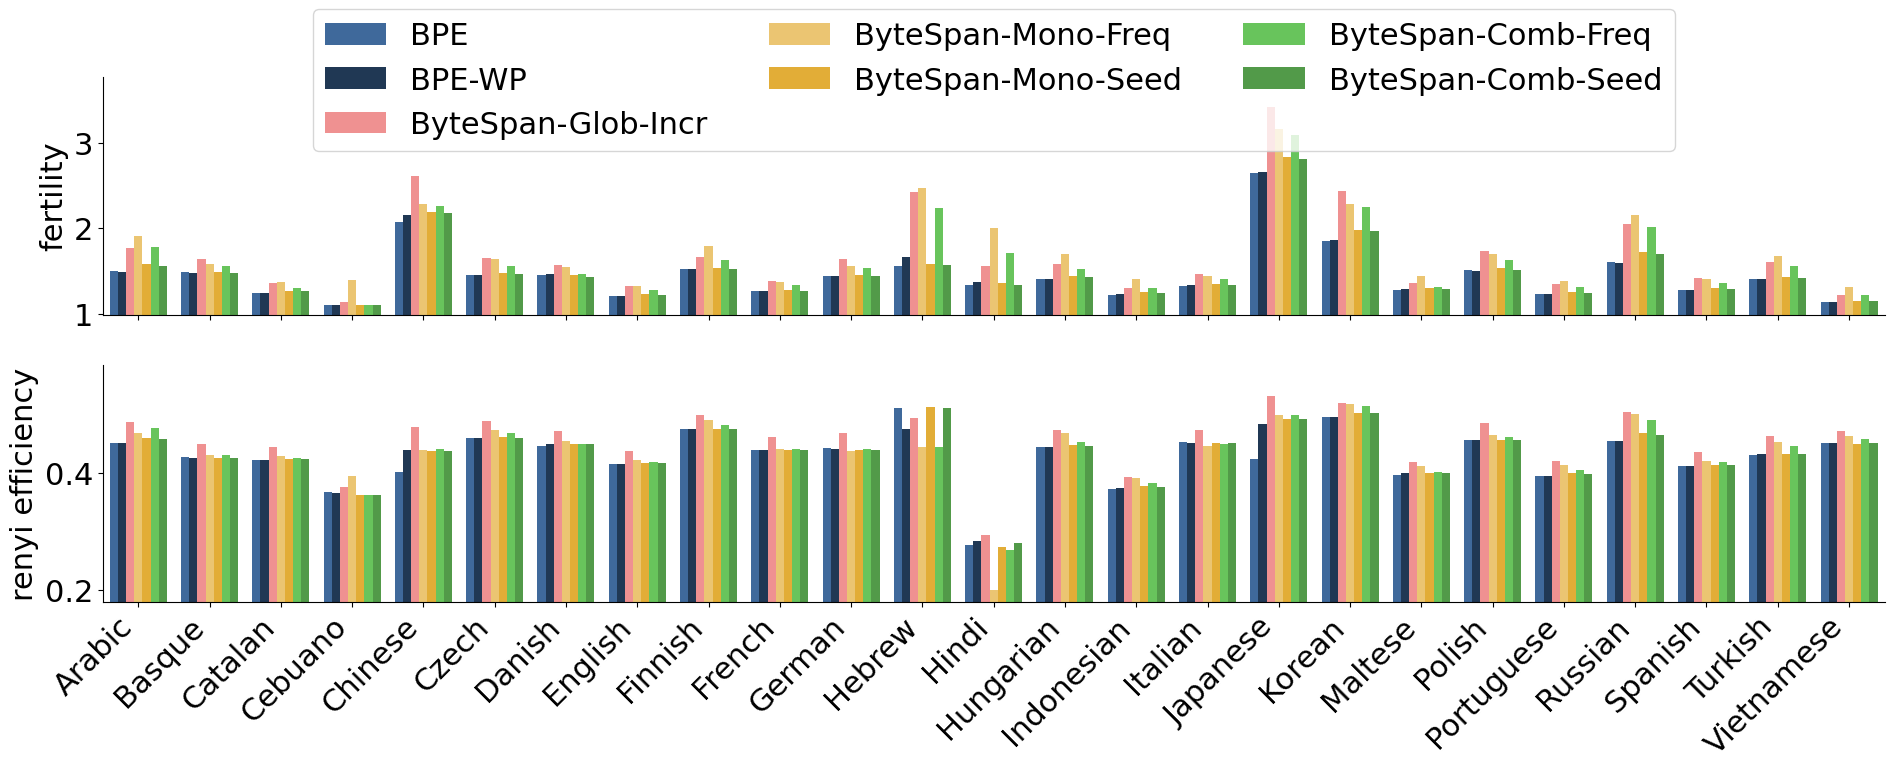
\includegraphics[width=\linewidth]{16InfoTok/multilingual.png}
        \caption{\bytespan tokenisers using surprisal.}
    \end{subfigure}
    \begin{subfigure}{0.98\linewidth}
        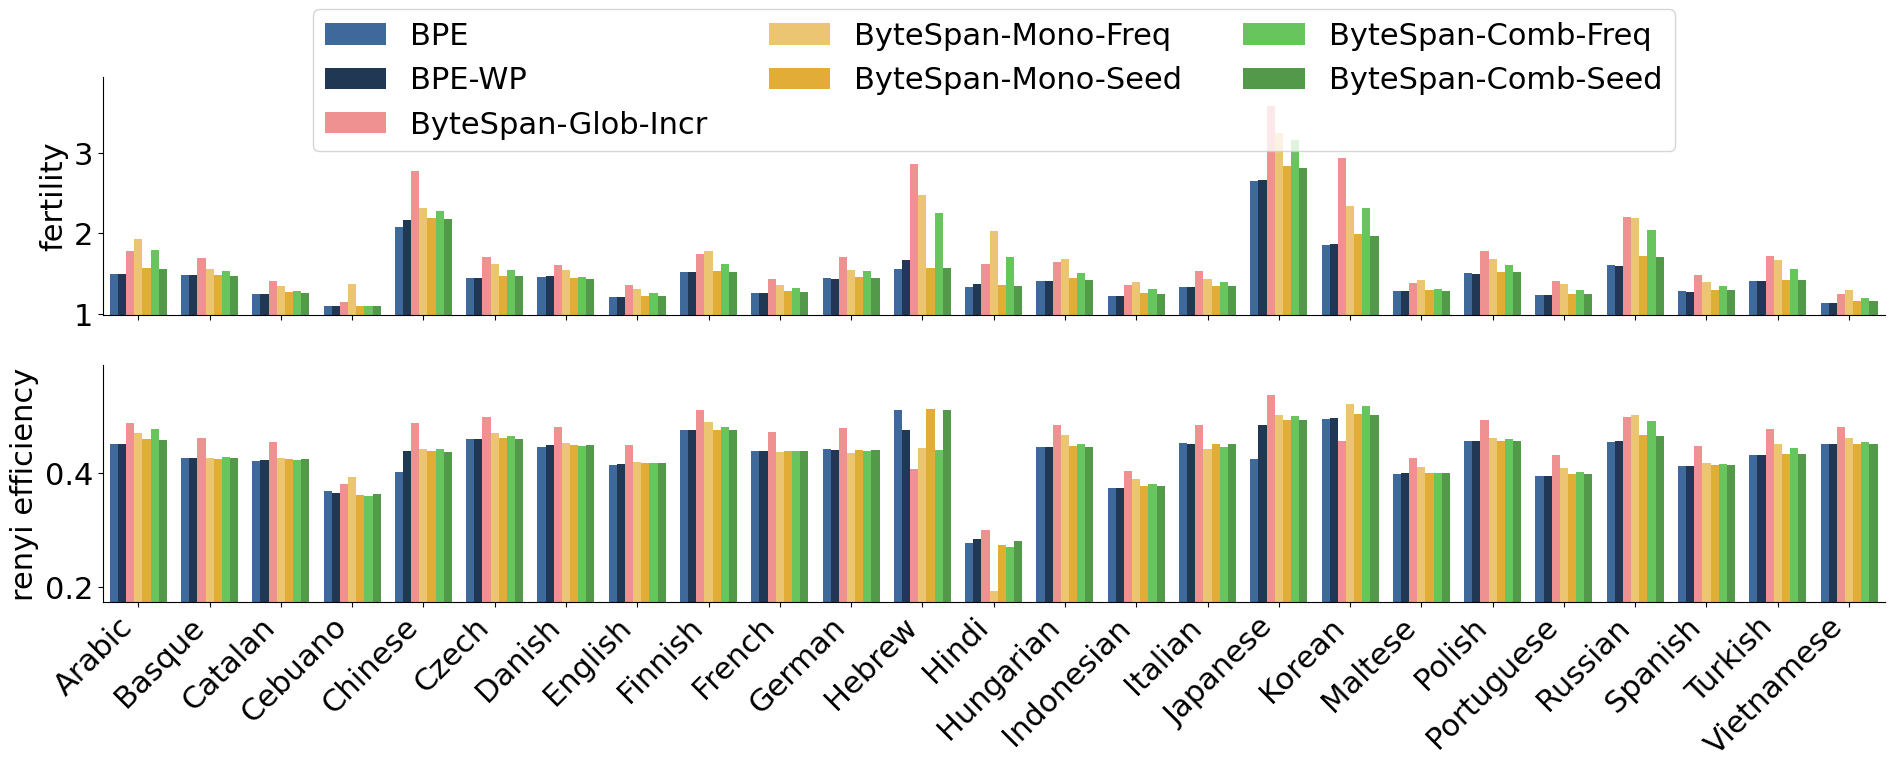
\includegraphics[width=\linewidth]{16InfoTok/multilingualentropy.png}
        \caption{\bytespan tokenisers using entropy.}
    \end{subfigure}
    \caption{Fertility and \renyi efficiency for each language in the \commoncorpus evaluation subset, comparing multilingual \bpe to the multilingual \bytespan tokenisers with a vocabulary size of \q{128}{\thousand}.}
    \label{fig:16-multilingual}
\end{figure}

\paragraph{Surprisal vs. entropy.}

For almost every measure, the tokenisers using \textbf{surprisal} achieve almost identical results to those using \textbf{entropy}. Comparing vocabularies, there is a very high overlap --- ranging from \q{85.7}{\percent} to \q{98.8}{\percent} --- suggesting that both measures of information identify similar byte spans. This is a similar result to the unsupervised word segmentation experiments in \cref{chapter:phonology}, where entropy and surprisal lead to similar segmentation results. In both experiments, these two statistics seem to be very closely-related measures of model uncertainty. %Thus, only report the \textbf{surprisal} scores are reported in this section. Below, the key findings are summarised.

\paragraph{Linguistic and cognitive alignment.}

The English \bytespan tokenisers achieve higher morphological alignment scores than \bpe and \bpewp for each vocabulary size but achieve lower scores on the cognitive plausibility metric. This indicates that morphological units in text can be successfully extracted using the surprisal from a byte-level model but that the number of splits may not correlate well with human performance in a lexical decision task. The results for \bpe and \bpewp mirror those of \citet{uzan-etal-2024-greed}, who found that using the vocabulary from \bpe but applying the WordPiece inference strategy led to higher morphological alignment but lower cognitive plausibility. In general, their results suggest a trade-off between these two measures, which can also be observed here with the \bytespan tokenisers. It is unclear which score is more desirable, although morphological alignment has long been hypothesised to be important for downstream use-cases (see e.g. \citet{gow-smith-etal-2022-improving}).

When comparing between the proposed constraints and learning methods, the global constraint achieves the highest morphological alignment score for all three vocabulary sizes (and due to the apparent trade-off, also the lowest cognitive plausibility score). This result contradicts qualitative analysis of the tokenisers; in many cases, such as the example phrase in \cref{fig:16-example}, the global constraint seems to segment the first few letters of a word individually and then the rest of the word as one token, since surprisal tends to fall towards the end of a word. This does not seem to align with English morphology and in most examples, the monotonic or combined constraints seem to produce more morphological segmentations. An investigation of how the morphological alignment score is calculated in the intrinsic benchmark reveals that it skips words \emph{unless all items in the gold segmentation of that word are contained in the vocabulary of the tokeniser}. For example, if a tokeniser's vocabulary does not contain the tokens \(\ex{ramp}, \ex{ant}, \ex{ly}\) then the word \ex{rampantly} is skipped. This can skew the score if a tokeniser's vocabulary does not contain many valid morphemes or stems, making comparison between tokenisers with different vocabularies difficult.

In order to explore this further, the \textbf{morphological coverage} of a tokeniser is defined as the percentage of words in the morphological data where all gold segments exist in the tokeniser's vocabulary (i.e, the percentage of the words used to calculate the alignment score for each tokeniser). The coverage in shown in \cref{fig:16-coverage}. Indeed, the tokenisers using the global constraint have much lower coverage, suggesting that the high alignment score is not comparable to the other tokenisers. This analysis reveals that the other \bytespan tokenisers have similar coverage to \bpe and \bpewp and still achieve higher morphological alignment, suggesting that they do produce a more linguistically motivated segmentation, with the combined constraint tokenisers achieving both high coverage and high alignment. 

\begin{figure}[!t]
    \centering
    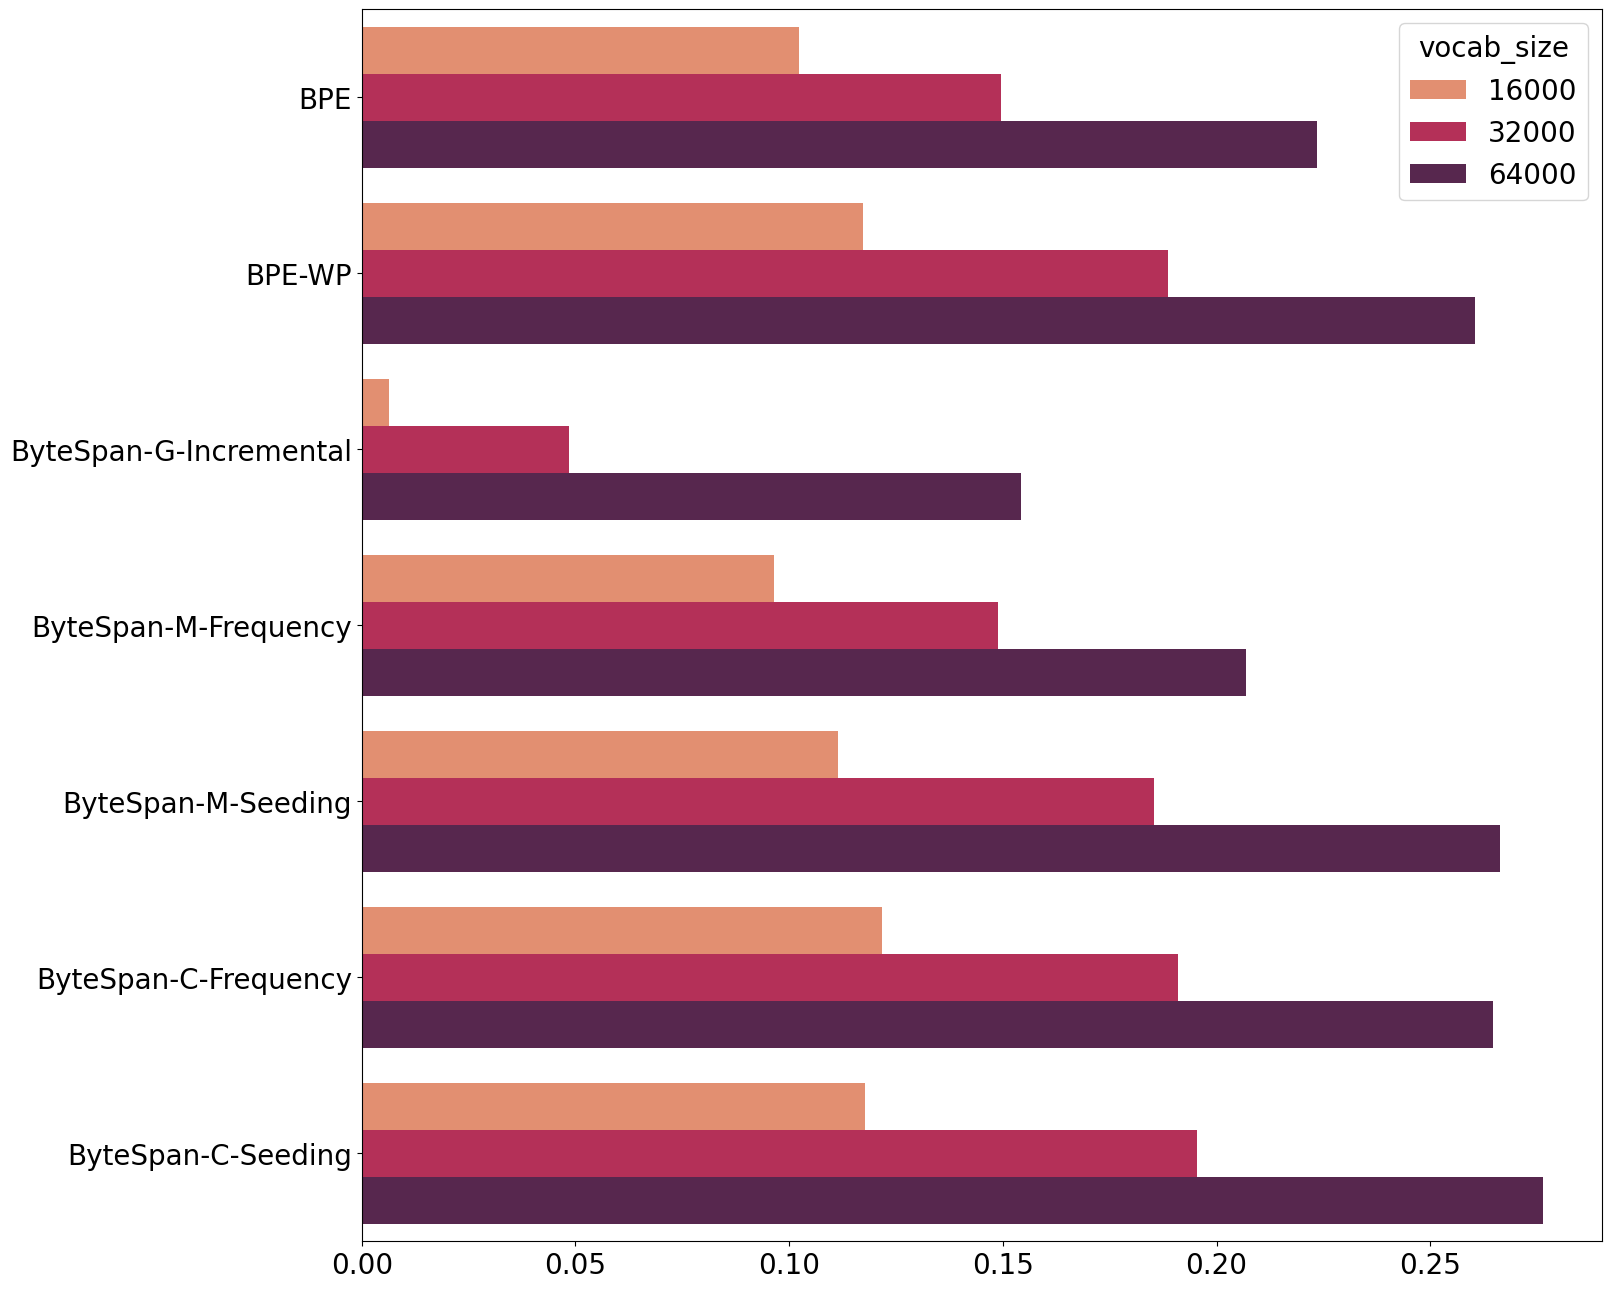
\includegraphics[width=0.95\linewidth]{16InfoTok/coverage.png}
    \caption{Morphological coverage of \bpe, \bpewp and the \bytespan tokenisers using surprisal.}
    \label{fig:16-coverage}
\end{figure}

\paragraph{Token distribution statistics.}

Besides those using the global constraint, the \bytespan tokeniser lead to higher \renyi efficiency scores than \bpe and \bpewp and very similar fertility scores across vocabulary sizes. This indicates that \bytespan leads to good compression while ensuring that the vocabulary space does not contain too many high-frequency and low-frequency tokens. Comparing between the incremental method and the seeding method for using \bytespan to learn a vocabulary, the seeding method improves fertility at the cost of \renyi efficiency, resulting in scores very similar to \bpewp. The fact that these tokenisers have similar token distribution statistics to \bpewp but maintain a higher morphological alignment score suggests that by using \bytespan to learn an initial vocabulary that is then supplemented by \bpe, the resulting vocabulary contains more morphologically-aligned tokens without sacrificing compression.

To investigate this further, token lengths can be compared. \cref{fig:16-distribution} shows the distribution of token lengths in the vocabularies of the \bpewp tokeniser and the two \bytespan tokenisers with the combined constraint for the largest vocabulary size. For all three tokenisers, the most common token lengths are \integer{4} and \integer{5}, but the frequency method leads to a tighter distribution around these lengths compared to \bpewp. The seeding method provides a balance by allowing \bpe to merge commonly occurring sequences identified by \bytespan, creating a distribution that more closely resembles the long tail of the \bpewp vocabulary.

In general, the global constraint does not lead to good compression. This is because, as observed in \cref{fig:16-example}, the first letters of words are highly unpredictable and so tend to be initially segmented at the character-level, even if long suffixes are compressed. The fact that this method learns long suffixes is also at odds with the longest-\textbf{prefix} inference method that is used. For example, for the largest tokeniser trained using this constraint, the token \ex{bonization} is learned but \ex{carbonization} is tokenised as \(\{\ex{carbon},\ex{ization}\}\) because the token \ex{carbon} also exists in the vocabulary. The monotonic and combined constraints seem to learn units across words so are not as negatively affected by this inference method.

\paragraph{Multilingual evaluation.}

The fertility and \renyi efficiency scores for each tokeniser across the \integer{25} languages in the training corpus are given in \cref{fig:16-multilingual}. Note that the fertility scores are higher for Chinese, Japanese and Korean because these languages are not delimited by whitespace in \commoncorpus, so pre-tokens consist of entire phrases. 

\begin{figure}[!t]
    \centering
    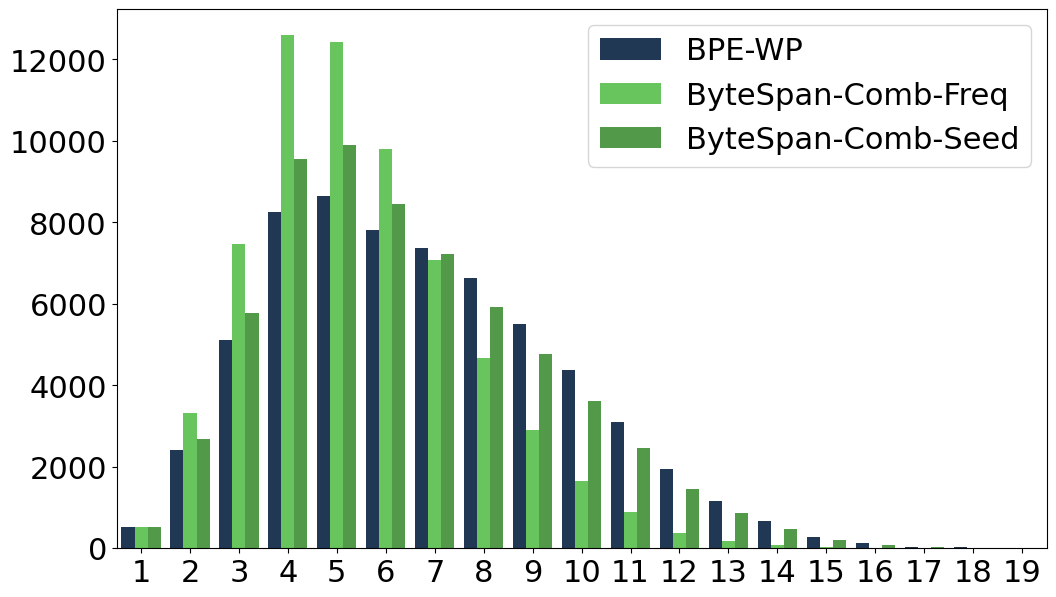
\includegraphics[width=0.95\linewidth]{16InfoTok/distribution.png}
    \caption{Distribution of token lengths comparing \bpewp to the \bytespan tokenisers using surprisal and the combined constraint with either the frequency method or the seeding method to learn the vocabulary. Vocabulary size is \q{64}{\thousand}.}
    \label{fig:16-distribution}
\end{figure}

Mirroring the English results, the \bytespan tokenisers score achieve higher \renyi efficiency scores but lower fertility for most languages. Out of the \bytespan tokenisers, the lowest fertility scores are achieved by the monotonic or combined constraints using the seeding method, whereas the incremental method and frequency method produce higher fertility scores. This difference is particularly pronounced for the languages in \commoncorpus with unique writing systems; Arabic, Chinese, Hebrew, Hindi, Japanese, Korean and Russian. It is possible that since the frequency method adds the top $|V|$ most frequent byte spans to the vocabulary, this will naturally bias towards orthographies shared by most of the corpus (in this case, subwords containing Latin characters). Similarly, as the incremental method gradually raises the global threshold $\thres_g$, if the byte-level LM struggles to predict rarer orthographies due to occurring less frequently in the data, the threshold may not add as many subwords from those languages. In the case of the frequency method, allowing \bpe to learn the remaining \q{50}{\percent} of the vocabulary seems to be an effective strategy, but \bpe is also implicitly biased by frequency.

\begin{figure}[!t]
    \centering
    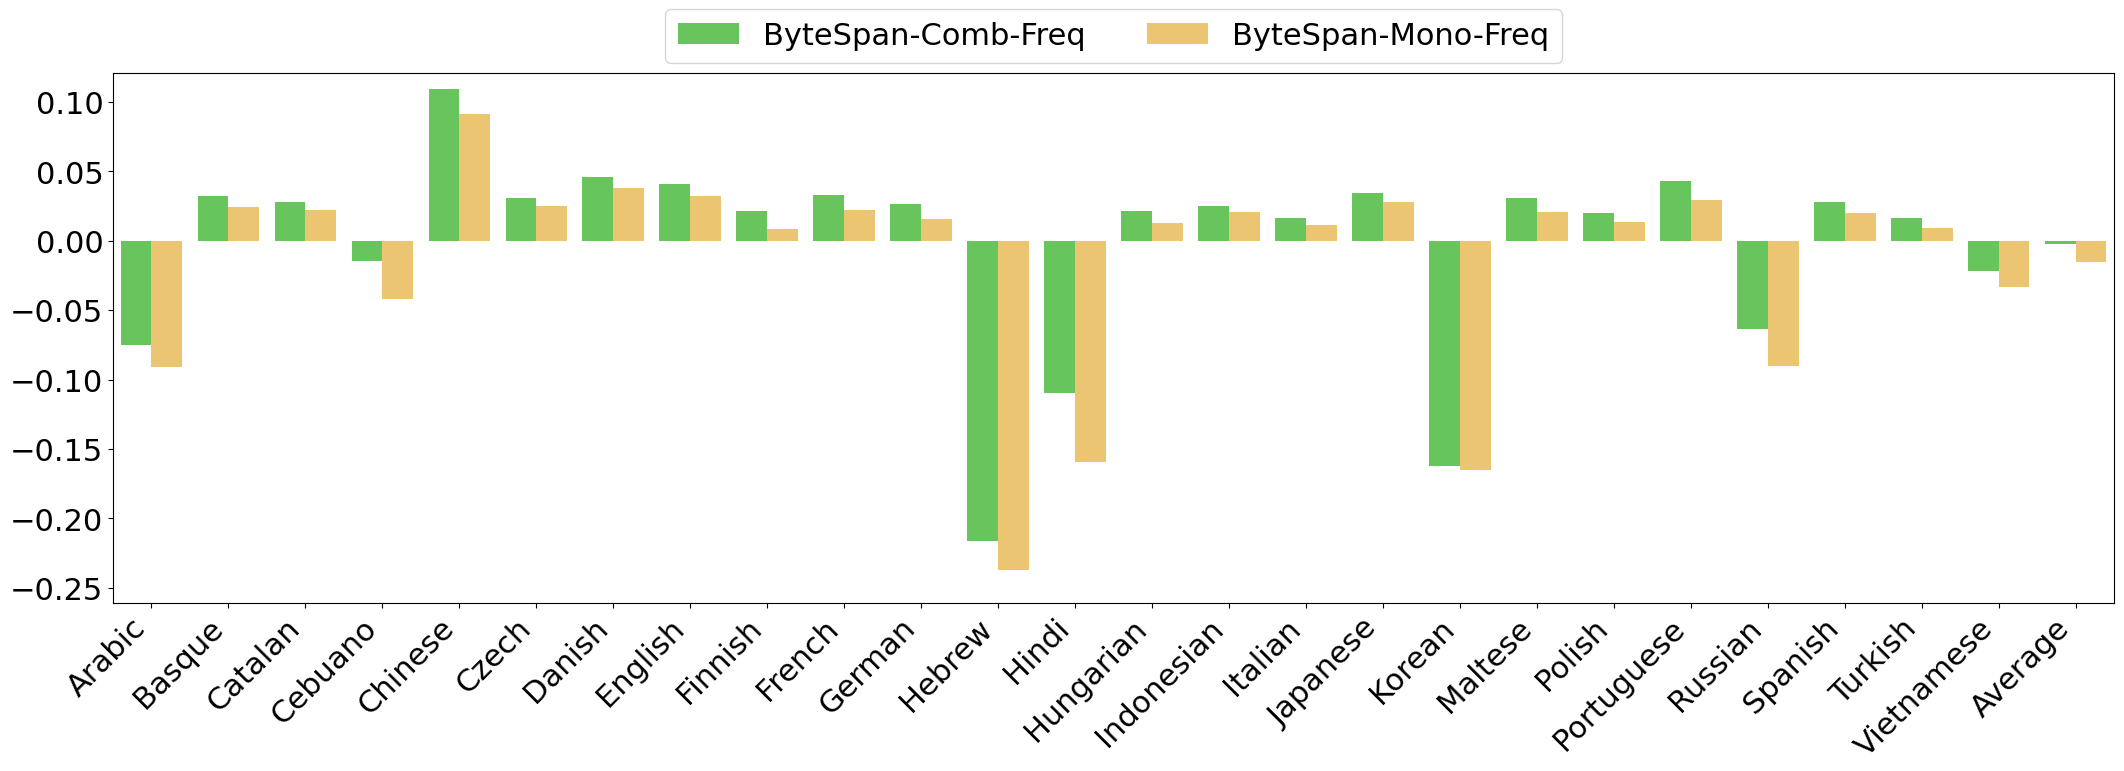
\includegraphics[width=0.9\linewidth]{16InfoTok/difference.png}
    \caption{Increase in fertility for each language when balancing added tokens across languages when training the multilingual \bytespan tokenisers with the frequency method. The tokenisers use surprisal as the byte-level measure and the vocabulary size is \q{128}{\thousand}. A decrease in fertility indicates better compression.}
    \label{fig:16-difference}
\end{figure}

One possible approach to this problem is considered. For the frequency method, instead of selecting the top $|V|$ most frequent discovered subwords across the whole dataset, the method can be adjusted to select the top $\frac{|V|}{L}$ most frequent discovered subwords for each language\footnote{Since subwords can appear in the frequency lists of multiple languages, tokens are added round-robin until the desired vocabulary size is met, which in practice can assign more than $\frac{|V|}{L}$ tokens from the languages with rarer orthographies.} (where $L$ is the number of languages). This guarantees that the rarer orthographies are assigned a dedicated portion of the final vocabulary. The effect of this adjustment on fertility is shown in \cref{fig:16-difference}. This approach seems to lead to the desired outcome; fertility decreases for most of the languages with unique orthographies (all but Chinese). By dedicating a portion of the vocabulary to these languages, the fertility does slightly rise for all Latin-script languages, but the average across languages is not affected (even slightly decreasing). 

\paragraph{Extrinsic evaluation.}

Extrinsic results are provided in \cref{tab:16-extrinsicresults}. Significance is calculated using a paired student t-test using the 67 task-level scores for \blimp and the \q{10}{\thousand} validation set scores for BPB with a significance value of $p<0.05$. The best \blimp score is achieved by the model trained with \bytespan using the monotonic constraint and frequency learning method and the word score is achieved by the model trained with \bytespan using the global constraint and incremental learning method. These are also the only two scores that are significantly different; all other comparisons do not achieve $p$-values below \integer{0.05}.The fact that the global constraint also led to poor intrinsic evaluation scores suggests that the intrinsic benchmark does predict language modelling capability, and also that creating a subword vocabulary using the global constraint does not help a model learn grammatical generalisations as well as the monotonic constraint. 

The BPB scores are also similar across all seven models, with three tokenisers all achieving the lowest (best) BPB of \integer{.824}. Again, the worst-scoring model is the one trained using \bytespan with the global constraint. Here, many scores are significantly different, although this is largely due to the high number of scores used in the t-test --- generally, all seven models achieve a very good fit over the validation set.

Overall, these extrinsic results suggest that the monotonic and combined constraints do not inhibit language modelling capabilities compared to \bpe. 

\begin{table}[t]
    \centering
    \footnotesize
    \begin{tabular}{cccccccc}
        \toprule
        Tokeniser & Constraint & Learning Method & \blimp & BPB \\
        \midrule
        \bpe & - & - & 78.7 &  .825 \\
        \bpewp & - & - & 78.7 & \textbf{.824} \\
        \bytespan & \red{Global} & Increment & 77.7 &  .843 \\
        \bytespan & \yellow{Monotonic} & Frequency & \textbf{79.4} & .832 \\
        \bytespan & \yellow{Monotonic} & Seeding & 78.7 & \textbf{.824} \\
        \bytespan & \green{Combined} & Frequency & 78.1 & .827 \\
        \bytespan & \green{Combined} & Seeding & 78.7 & \textbf{.824} \\
        \bottomrule
    \end{tabular}
    \caption{Extrinsic evaluation results comparing \bpe and \bpewp to the \bytespan tokenisers using surprisal. The vocabulary size for all tokenisers is \q{64}{\thousand}. Scores are given to three significant figures, with the best score for each vocabulary size marked in \textbf{bold}.}
    \label{tab:16-extrinsicresults}
\end{table}

\section{Discussion}\label{sec:16-discussion}

\bytespan achieves a balance between dynamic patching approaches and the computational benefits of a fixed vocabulary size. Intrinsic evaluation in English reveals that this approach improves morphological alignment and \renyi efficiency compared to \bpe and \bpewp while retaining similar levels of compression. Extrinsic results reveal that training models using \bytespan tokenisers do not inhibit grammatical generalisation and language modelling compared to \bpe, but that the global constraint does. Whereas \citet{pagnoni2024byte} only used entropy in their study, here, surprisal is found to be an effective informative signal for grouping predictable bytes. As surprisal is cheaper to compute than entropy, this could lead to efficiency gains for dynamic patching approaches that require information to be calculated at every byte during training. Further work could explore information-based tokenisation with alternative information signals, such as the probability of whitespace tokens, mimicking the utterance boundary probability cue used for word segmentation in \cref{chapter:phonology} and in prior models \citep{christiansen1998learning}.

Multilingual evaluation reveals that the information-based approach struggles with languages whose writing systems are less represented in the data, but that using \bytespan to seed an initial vocabulary before applying \bpe addresses a gap in compression for these languages. The frequency method for learning a vocabulary may implicitly lead to the vocabulary being biased towards more the more frequent orthographies found in the training data, but that by adjusting the vocabulary-learning method to force the same number of subwords to be added for each language, fertility can be improved for languages with unique orthographies. In general, \bytespan still relies on grouping contiguous bytes based on the predictions from a byte-level LM, which may not identify useful subwords for non-concatenative languages or right-to-left languages like Arabic and Hebrew. By using bytes as the fall-back representation, the encoding bias of UTF-8 is also perpetuated, which on average assigns more bytes per character for non-Latin-script languages. Future work should incorporate more balanced byte-level schemes, such as MYTE, a morphologically-driven byte encoding \citep{limisiewicz-etal-2024-myte}.

Although \bytespan is parameter-free for certain combinations of constraints and vocabulary-learning methods, the combined constraint and \textbf{seeding method} both use hyper-parameters which not thoroughly explored here ($p=50\%$ is set for the seeding method and $\thres_g$ is set to the 30th-percentile for the combined constraint). These should be explored further in future work. Future work could also explore the use of an \textbf{approximate} monotonic constraint (using $H(\ch_t) - H(\ch_{t-1}) < \thres_m$ instead of $H(\ch_t) - H(\ch_{t-1}) < 0$). This was proposed by \citet{pagnoni2024byte} and could provide an alternative mechanism of dealing with the instability of the monotonic constraint at near-zero values for surprisal and entropy. Finally, the tokenisers implemented in this chapter use longest-prefix matching for inference, but the learned vocabularies are compatible with other inference strategies, such as longest-suffix matching \citep{jacobs2022lost}.

% as these could impact the predictions extracted from a byte-level model. Future work could explore balancing writing systems as well as languages when choosing a tokeniser using this method, or training separate, smaller byte-level models for each language. Our method also uses an autoregressive model, which may not be appropriate for right-to-left writing systems and languages with non-concatenative morphology. Further work might explore the effect of adding non-contiguous information thresholds for non-concatenative morphologies.

% In an initial experiment, we found that one of our tokenisers did not achieve significantly different results compared to \bpe using a minimal-pair linguistic judgement task (see \cref{app:blimp}). 

% - Our method uses entropy of current token, patches does next token, perhaps would have gotten full words more often with next-entropy.

% The proposed method of training a tokeniser based  on entropy or surprisal thresholds achieves a balance between adaptive or dynamic segmentation approaches and the computational benefits of a fixed \(\mathcal{V}\). Using a LM's predictions to choose a tokeniser's vocabulary is not a novel proposal. In fact, the WordPiece objective was originally to maximise a dataset's likelihood under an \ngram model, with predictions re-estimated after each merge \citep{schuster-nakajima-2012-voice}. The modern WordPiece objective given in \cref{eq:wp_obj}, which purportedly optimises for mutual information, also greedily optimises a unigram model's likelihood of the dataset. Our proposed method does not require re-estimation and needs to train a transformer-based LM only once to produce higher-quality predictions. The  model-agnostic nature of our method, which modularises dynamic tokenisation from architectures, might provide a structured and computationally-efficient framework for other architecture that do not inherently handle dynamic segmentation (e.g., simple Transformers, feed-forward models) and might also be advantageous in resource-constrained settings (e.g., performing dynamic segmentation on edge devices).  Future work in dynamic information-driven tokenisation might  integrate further ideas of dynamic tokenisation into this modularised setting, such as learning monotonically decreasing units first rather than setting a set threshold, or using  a simple unigram model to evaluate and starts with a large vocabulary that is subsequently pruned.

%\Zeb{Prefix-first strategy of unigram may not be appropriate for this approach. Could also look at .}\Zeb{Maybe mention UnigramLM bases selection of tokens on how they are used in a language model but uses a simple unigram model to evaluate and starts with a large vocabulary that is pruned.} 

\section{Summary}

This chapter has primarily addressed Research Question \ref{question:rq3}, by presenting \bytespan, a novel method for learning a subword vocabulary using the predictions of a byte-level LM, inspired by the success of unsupervised methods using phoneme LMs on the word segmentation task presented in \cref{chapter:phonology}. By grouping contiguous sequences of predictable bytes using one of three constraints, \bytespan tokenisers have efficient vocabularies with a higher morphological alignment than \bpe and \bpewp on English evaluation sets, with the monotonic constraint generally being more effective than the global constraint. In the multilingual setting, \bytespan tokenisers result in similar compression rates to \bpe but some methods struggle to compress languages with unique orthographies. Hypothesising that this could be due to the frequency-based vocabulary-learning method, an alternative method that balances the vocabulary by language was found to counteract this effect.

In general, \bytespan provides a novel method for learning subwords with parallels to word segmentation and patching, all while keeping the benefits of learning a fixed-size vocabulary for efficient language modelling. This work demonstrates how analytical research into alternative input representations can produce new insights for practical language modelling --- in this thesis, phoneme LMs trained on child-directed speech used for word segmentation has led to new insights into both static subword tokenisation and could also improve dynamic patching approaches. 

% This could feed into explorations of information in lexical unit extraction that may improve future static tokenisers and dynamic patching approaches.

% ===========
% LIMITATIONS
% ===========
% \section*{Limitations}

% In this study we propose novel methods for learning a subword vocabulary but only use one inference method for applying the tokenisers; the longest-prefix method of WordPiece. Future work could explore the use our learned vocabularies with alternative inference methods, such as longest-suffix matching \citep{jacobs2022lost}.

% The experiments reported in the paper only utilise one type of Transformer models, although preliminary work utilised a 5-gram model. Further work might explore the scaling properties of the byte-level model. Our evaluation largely focused on English, although we do explore a multilingual setting. In our multilingual setting we are restricted to token distribution statistics due to limited evaluation resources available for these other languages, although there are individual pipelines for individual languages (e.g., \citet{gazit2025splinteringnonconcatenativelanguagesbetter} uses lexical decision data to evaluate Hebrew tokenisers).

% \Zeb{WordPiece model could be a limitation since our vocabulary starts with three copies of each byte, although this becomes relatively less of a waste with larger vocabulary sizes, and our \renyi efficiency is still better than \bpe in most cases}

% \paragraph{Reproducibility.}

% We release all experimental artefacts as a collection on the Hugging Face Hub at \href{https://huggingface.co/InfoTokenizers}{huggingface.co/InfoTokenizers}: (i) the byte-level versions of the two datasets; (ii) the subsets of each dataset used to train the byte-level models, extract predictions and evaluate the resulting tokenisers; (iii) the byte-level surprisal and entropy for each dataset; (iv) the \bpe, \bpewp and \bytespan tokenisers used in our experiments; (v) all model checkpoints. Our codebase is available at \href{https://github.com/codebyzeb/bytespantokenization}{github.com/codebyzeb/bytespantokenization}.\looseness=-1
